\documentclass{beamer}

% Anleitung zur Klasse beamer unter: http://www.ctan.org/tex-archive/macros/latex/contrib/beamer/doc/beameruserguide.pdf

%
% Einbinden von LaTeX-Paketen
%

% Zeichenkodierung in diesem Dokument ist UTF-8
\usepackage[utf8x]{inputenc}
% Sprache des Dokuments ist Deutsch (neue Rechtschreibung)
%\usepackage{ngerman}

% es sollen Grafiken eingebunden werden
\usepackage{graphicx}

\usepackage{subfig}

% Design Warsaw
\usetheme{Warsaw}

% abgedeckte Elemente auf einer Folie werden transparent gemacht
\setbeamercovered{transparent}

%% zu Beginn jeder Section wird folgende Folie eingefügt
%\AtBeginSection[]
%{
% \begin{frame}{Übersicht}
%  % Übersicht: aktuelle Section (hervorgehoben) mit ubsections im Kontext anderer Sections
%  \tableofcontents[currentsection,currentsubsection,hideothersubsections]
% \end{frame}
%}

%% zu Beginn jeder Subsection wird folgende Folie eingefügt
%\AtBeginSubsection[]
%{
% \begin{frame}{Übersicht}
%  % Übersicht: aktuelle Section (hervorgehoben), aktuelle Subsection (hervorgehoben) im Kontext der anderen Subsections
%  \tableofcontents[currentsection,currentsubsection,subsectionstyle=show/shaded/hide]
% \end{frame}
%}


\title{I2C am RaspberryPi}
\author{Guido Schmitz}
\date{Pi And More // 23. August 2012}



\begin{document}

% Titelfolie
\begin{frame}[plain]
 \titlepage
\end{frame}

\begin{frame}{Overview}
 \tableofcontents
\end{frame}


\section{Was ist I2C?}

\begin{frame}{Grundlegendes}
 \begin{itemize}
  \item I2C = Inter-Integrated Circuit
   \begin{itemize}
    \item sprich: "I Quadrat C" oder "I Zwei C" oder "I squared C"
    \item oder auch: TWI = two wire interface (nur anderer Name)
    \item oder auch: SMBus (nur marginal technisch anders)
   \end{itemize}
  \item serieller Datenbus
   \begin{itemize}
    \item seriell = eine Datenleitung, darauf alles nacheinander
    \item Bus = mehrere Teilnehmer an gemeinsamen Leitungen
   \end{itemize}
 \end{itemize}
\end{frame}

\subsection{Physikalisch}

\begin{frame}{Leitungen}
 \begin{itemize}
  \item zwei Leitungen
   \begin{itemize}
    \item Serial Data Line (SDA)
    \item Serial Clock Line (SCL)
   \end{itemize}
  \item ein Master, mehrere Slaves (max. 112)
 \end{itemize}
 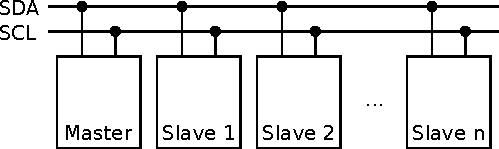
\includegraphics[width=\textwidth]{bus}
\end{frame}

\begin{frame}{Elektrisch}
 \begin{itemize}
  \item geimensame Referenzspannung Ground / 0V\\(auch: GND, Common, COM)
  \item Versorgungsspannung Vcc (auch: Vdd) / hier: 3.3V
    \begin{alertblock}{Achtung}
     Viele Komponenten arbeiten mit 5V Versorgungsspannung!\\
     5V Spannung kann 3.3V Komponenten zerstören!\\
     (insbesondere das RaspberryPi)
    \end{alertblock}
  \item aber: I2C unkritisch (wenn richtig angeschlossen)
  \item Ground bis Vcc OK (max. 0.5V darüber hinaus!)
 \end{itemize}
\end{frame}

\begin{frame}{Pegel}
 \begin{itemize}
   \item Spannung = Informationszustand
    \begin{itemize}
      \item 0V = Low-Pegel = logisch 0
      \item 3.3V = High-Pegel = logisch 1
    \end{itemize}
  \item Spannung muss nicht genau passen
  \item Ganz grob gesagt: unteres Drittel Low (0V-1.1V), oberes Drittel High (2.2V-3.3V)
  \item bei 5V Komponenten: Low 0V-1.7V, High 3.3V-5V (passt!)
 \end{itemize}
\end{frame}

\begin{frame}{Pegelerzeugung}
 \begin{itemize}
   \item I2C-Bus wird durch Pull-Up Widerstände auf 3.3V gehalten
   \item Pull-Up Widerstände hochohmig (mehrere $k\Omega$),\\im Raspberry Pi integriert
   \item Komponenten beeinflussen Leitung erstmal nicht\\(Open-Collector, Open-Drain)
   \item Komponenten können Leitung auf Ground ziehen
 \end{itemize}
\end{frame}

\subsection{Logisch}

\begin{frame}{Kommunikation}
 \begin{itemize}
 \end{itemize}
\end{frame}

\section{Wie benutzen wir I2C?}

\end{document}
